% \pause
% \alert{text}
% \uncover<5->{\item foo}  al posto di \item
%\includegraphics[height=1cm]{moogle}
\documentclass{beamer}
\usepackage{graphicx}
%\usepackage{bcprules}
\usepackage{verbatim}
\usepackage{amsmath}
\usepackage{amssymb}
\usepackage{stmaryrd}
\usepackage{bussproofs}
\usepackage{bbding}
\usepackage{ dsfont }
%\usepackage{ebproof}
%\usepackage{stmaryrd}

% !TEX root = ../main.tex
%\usepackage{ulem}
%\input{\macrospath/ben-macros-diagrams.tex}
%\usepackage[usenames,dvipsnames,svgnames,table]{xcolor}

\newcommand{\sem}[1]{[\![#1]\!]}

%%%%%%%
%% LATEX SHORTCUTS
%%%%%%%
\newcommand{\ignore}[1]{}
\newcommand{\sep}{\hspace*{0.5cm}}
\newcommand{\ms}{\medskip}
\newcommand{\mathintitle}[2]{\texorpdfstring{#1}{#2}}
\newcommand{\colspace}{@{\hspace{.5cm}}}
\newcommand{\myinput}[1]{\ifthenelse{\boolean{withimages}}{\input{#1}}{}}
\newcommand{\spc}{@{\hspace{.5cm}}}

% for references
\newcommand{\reflemma}[1]{Lemma~\ref{l:#1}}
\newcommand{\reflemmap}[2]{Lemma~\ref{l:#1}.\ref{p:#1-#2}}
\newcommand{\reflemmaeq}[1]{{L.\ref{l:#1}}}
\newcommand{\refcorollary}[1]{Corollary~\ref{c:#1}}
\newcommand{\refcorollaryp}[2]{Corollary~\ref{c:#1}.\ref{p:#1-#2}}
\newcommand{\refth}[1]{Theorem~\ref{th:#1}}
\newcommand{\refthm}[1]{Theorem~\ref{thm:#1}}
\newcommand{\reftm}[1]{Theorem~\ref{tm:#1}}
\newcommand{\refprop}[1]{Proposition~\ref{prop:#1}}
\newcommand{\refsect}[1]{Sect.~\ref{sect:#1}}
\newcommand{\reftab}[1]{Tab.~\ref{tab:#1}}
\newcommand{\refeq}[1]{(\ref{eq:#1})}
\newcommand{\reffig}[1]{Fig.~\ref{fig:#1}}
\newcommand{\refcoro}[1]{Corollary~\ref{coro:#1}}

% macro for cases in proofs
%\newcommand{\case}[1]{{\bf Case #1.}}
%\newcommand{\casealt}[1]{{\bf #1.}}
%\newcommand{\caselight}[1]{\textit{#1}}

%%%%%%%
%% ABBREVIATIONS
%%%%%%%
\newcommand{\ie}{\textit{i.e.}}
\newcommand{\eg}{\textit{e.g.}}
\newcommand{\ih}{\textit{i.h.}}
\newcommand{\lat}{\mbox{$\lambda$-term}}

\newcommand{\linlogic}{linear logic}
\newcommand{\Linlogic}{Linear logic}
\newcommand{\pn}{proof net}
\newcommand{\Pn}{Proof net}
\newcommand{\pns}{proof nets}
\newcommand{\Pns}{Proof nets}

\newcommand{\wlhr}{WLHR}

\newcommand{\activep}{substitutive}
\newcommand{\Activep}{Substitutive}
\newcommand{\inactivep}{applicative}
\newcommand{\Inactivep}{Applicative}

%%%%%%%
%% TEXT FORMATTING
%%%%%%%
\newcommand{\deff}[1]{\textbf{#1}}
\newcommand{\boldemph}[1]{\textbf{#1}}
\newcommand{\scol}{\mathbin;}

\newcommand{\underlinecolor}[2]{{\color{#1}\underline{\black{#2}}\color{black}}}
\newcommand{\overlinecolor}[2]{{\color{#1}\overline{\black{#2}}\color{black}}}

\newcommand{\undlinered}[1]{\underlinecolor{red}{#1}}
\newcommand{\ovlinered}[1]{\overlinecolor{red}{#1}}

\newcommand{\red}[1]{{\color{red} {#1}}}
\newcommand{\blue}[1]{{\color{blue} {#1}}}
\newcommand{\brown}[1]{{\color{brown} {#1}}}
\newcommand{\green}[1]{{\color{green} {#1}}}
\newcommand{\darkgreen}[1]{{\color{green!50!black} {#1}}}
\newcommand{\black}[1]{{\color{black} {#1}}}
\newcommand{\purple}[1]{{\color{purple} {#1}}}
\newcommand{\orange}[1]{{\color{orange} {#1}}}

\newcommand{\ben}[1]{{\red{#1}}}
%\renewcommand{\ben}[1]{{#1}}
\newcommand{\bben}[1]{\sout{{\ben{#1}}}}
\newcommand{\cben}[2]{{\red{#2}}}
%\renewcommand{\cben}[2]{{#2}}
\newcommand{\pablo}[1]{{\darkgreen{#1}}}
%\renewcommand{\pablo}[1]{#1}
\newcommand{\cpablo}[2]{{\darkgreen{#2}}}
%\renewcommand{\cpablo}[2]{#2}
\newcommand{\damiano}[1]{{\blue{#1}}}
\newcommand{\cdamiano}[2]{{\blue{#2}}}
\newcommand{\claudio}[1]{{\purple{#1}}}
\newcommand{\cclaudio}[2]{{\purple{#2}}}


%%%%%%%
%% GENERIC MATH
%%%%%%%
\newcommand{\defeq}{\mathrel{:=}}
\newcommand{\grameq}{\mathrel{::=}}
\newcommand{\set}[1]{\{#1\}}
\newcommand{\disunion}{\uplus}
\newcommand{\card}[1]{\# #1}
\newcommand{\nat}{\mathbb{N}}
\newcommand{\size}[1]{|#1|}
\newcommand{\dummyarg}{\cdot}
\newcommand{\LeftRightarrow}{\Lleftarrow\!\!\!\!\Rrightarrow}

%%%%%%%
%% SYMBOLIZED LETTERS
%%%%%%%
\newcommand{\db}{{\tt dB}}
\newcommand{\dbv}{{\tt dBv}}
\newcommand{\lssym}{{\tt ls}}
\newcommand{\ls}{{\tt ls}}
\newcommand{\vartt}{{\tt var}}
\newcommand{\gc}{{\tt gc}}
\newcommand{\Bsym}{{\tt B}}
\newcommand{\lsvsym}{{\tt lsv}}
\newcommand{\vsym}{{\tt v}}
\newcommand{\tX}{\mathtt X}
\newcommand{\amsym}{{\tt am}}
\newcommand{\lamsym}{\l}
\newcommand{\apsym}{@}
\newcommand{\updsym}{u}
\newcommand{\varsym}{v}
\newcommand{\admsym}{c}
\newcommand{\noadmsym}{p}
\newcommand{\mulsym}{m}
\newcommand{\expsym}{e}
\newcommand{\isym}{{\mathtt i}}
\newcommand{\bsym}{{\mathtt b}}

%%%%%%%
%% LINEAR SUBSTITUTION CALCULUS
%%%%%%%
\newcommand{\lsc}{LSC}
\newcommand{\wlsc}{WLSC}
\newcommand{\wlscname}{{\tt Name}}
\newcommand{\wlscvaluelr}{{\tt Value}^{\tt LR}}
\newcommand{\wlscvaluerl}{{\tt Value}^{\tt RL}}
\newcommand{\wlscneed}{{\tt Need}}

\newcommand{\llsub}{\l_{lsub}}
\renewcommand{\l}{\lambda}
\newcommand{\isub}[2]{\{#1/#2\}}
\renewcommand{\isub}[2]{\{#1{\shortleftarrow}#2\}}
\newcommand{\esub}[2]{[#1/#2]}
\renewcommand{\esub}[2]{[#1{\shortleftarrow}#2]}
\newcommand{\fv}[1]{{\tt fv}(#1)}
\newcommand{\varsplit}[3]{#1_{[#3]_{#2}}}

%%%%%%%
%% REWRITING RELATIONS
%%%%%%%
% basic macros
\newcommand{\rootRew}[1]{\mapsto_{#1}}
\newcommand{\Rew}[1]{\rightarrow_{#1}}

% call-by-name root rules
\newcommand{\rtodb}{\rootRew{\db}}
\newcommand{\rtols}{\rootRew{\lssym}}
\newcommand{\rtolsc}[1]{\stackrel{#1}{\mapsto}_\lssym}

% call-by-value root rules
\newcommand{\rtodbv}{\rootRew{\db\vsym}}
\newcommand{\rtolsv}{\rootRew{\lssym\vsym}}
\newcommand{\rtolsvp}{\rootRew{\lssym\vsym'}}
\newcommand{\rtolsvc}[1]{\stackrel{#1}{\mapsto}_{\lssym\vsym}}

% call-by-name (weak linear head reduction)
\newcommand{\rtowhls}{\rtols} % this one is redundant but used in a proof
\newcommand{\towhl}{\stackrel{\mathtt{wh}}{\multimap}}
\newcommand{\towhldb}{\stackrel{\mathtt{wh}}{\multimap}_\db}
\newcommand{\towhlls}{\stackrel{\mathtt{wh}}{\multimap}_\lssym}
\renewcommand{\towhl}{\togen}
\renewcommand{\towhldb}{\togenm}
\renewcommand{\towhlls}{\togene}
\newcommand{\towhls}[1][\ast]{\overset{\mathtt{wh}}{\multimap}\!\!{}^{#1}}

% call-by-value (super-strategy)
\newcommand{\towhlv}{\multimap_\vsym}

% non-strict call-by-value
\newcommand{\towhlcek}{\stackrel{\mathtt{ns}}{\multimap}_\vsym}
\newcommand{\towhlcekdb}{\stackrel{\mathtt{ns}}{\multimap}_\dbv}
\newcommand{\towhlcekls}{\stackrel{\mathtt{ns}}{\multimap}_\lsvsym}
\renewcommand{\towhlcek}{\togen}
\renewcommand{\towhlcekdb}{\togenm}
\renewcommand{\towhlcekls}{\togene}


% strict call-by-value
\newcommand{\towhllam}{\stackrel{\mathtt{s}}{\multimap}_\vsym}
\newcommand{\towhllamdb}{\stackrel{\mathtt{s}}{\multimap}_\dbv}
\newcommand{\towhllamls}{\stackrel{\mathtt{s}}{\multimap}_\lsvsym}
\renewcommand{\towhllam}{\togen}
\renewcommand{\towhllamdb}{\togenm}
\renewcommand{\towhllamls}{\togene}


% call-by-need
\newcommand{\towhlsam}{\stackrel{\mathtt{nd}}{\multimap}}
\newcommand{\towhlsamdb}{\stackrel{\mathtt{nd}}{\multimap}_\db}
\newcommand{\towhlsamls}{\stackrel{\mathtt{nd}}{\multimap}_\lsvsym}
\renewcommand{\towhlsam}{\togen}
\renewcommand{\towhlsamdb}{\togenm}
\renewcommand{\towhlsamls}{\togene}


% reduction rules for oriented structural equivalence 
\newcommand{\tostructrev}{\Lleftarrow}
\newcommand{\tostructsym}{\LeftRightarrow}
\newcommand{\tostructrevgc}{\tostructrev_{\structrulegc}}
\newcommand{\tostructrevdup}{\tostructrev_{\structruledup}}
\newcommand{\tostructrevap}{\tostructrev_{\structruleap}}
\newcommand{\tostructreves}{\tostructrev_{\structrulees}}
\newcommand{\tostructrevcom}{\tostructrev_{\structrulecom}}

% generic linear rewriting
\newcommand{\esym}{{\mathtt e}}
\newcommand{\msym}{{\mathtt m}}
\newcommand{\rtogenm}{\mapsto_\msym}
\newcommand{\rtogene}{\mapsto_\esym}
\newcommand{\togen}{\multimap}
\newcommand{\togenm}{\multimap_\msym}
\newcommand{\togene}{\multimap_\esym}
\newcommand{\togenep}{\multimap_{\esym'}}
\newcommand{\togenx}{\multimap_{\mathtt x}}

\newcommand{\togenpar}[1]{\stackrel{#1}{\multimap}}

\newcommand{\tom}{\Rew{\msym}}
\newcommand{\toe}{\Rew{\esym}}

% miscellaneous rewriting relations
\newcommand{\toam}{\Rew{\amsym}}

%%%%%%%
%% EQUIVALENCES
%%%%%%%
\newcommand{\alphaequiv}{=_\alpha}
\newcommand{\eqstruct}{\equiv}
\newcommand{\tostruct}{\eqstruct}
\newcommand{\tostructgc}{\tostruct_{gc}}
\newcommand{\tostructgcv}{\tostruct_{gcv}}
\newcommand{\tostructdup}{\tostruct_{dup}}
\newcommand{\tostructap}{\tostruct_{@}}
\newcommand{\tostructapl}{\tostruct_{@l}}
\newcommand{\tostructapr}{\tostruct_{@r}}
\newcommand{\tostructes}{\tostruct_{[\cdot]}}
\newcommand{\tostructcom}{\tostruct_{com}}
\newcommand{\structrulegc}{gc}
\newcommand{\structrulegcv}{gcv}
\newcommand{\structruledup}{dup}
\newcommand{\structruleap}{@}
\newcommand{\structruleapl}{@l}
\newcommand{\structruleapr}{@r}
\newcommand{\structrulees}{[\cdot]}
\newcommand{\structrulecom}{com}

\newcommand{\eqmam}{\equiv_{\tiny \mbox{MAM}}}
\newcommand{\eqmamsym}{\LeftRightarrow}
\newcommand{\eqcekd}{\equiv}
\newcommand{\eqcekdsym}{\LeftRightarrow}
\newcommand{\eqcekdapl}{\eqcekd_{\structruleapl}}
\newcommand{\eqcekdapr}{\eqcekd_{\structruleapr}}
\newcommand{\eqcekdcom}{\eqcekd_{\structrulecom}}
\newcommand{\eqcekdes}{\eqcekd_{\structrulees}}


%%%%%%%
%% TERMS AND VARIABLES
%%%%%%%
% terms
\newcommand{\tm}{t}
\newcommand{\tmtwo}{u}
\newcommand{\tmthree}{w}
\newcommand{\tmfour}{r}
\newcommand{\tmfive}{q}
\newcommand{\tmsix}{p}

% terms with prime
\newcommand{\tmp}{\tm'}
\newcommand{\tmtwop}{\tmtwo'}
\newcommand{\tmthreep}{\tmthree'}
\newcommand{\tmfourp}{\tmfour'}
\newcommand{\tmfivep}{\tmfive'}

% terms with double prime
\newcommand{\tmpp}{\tm''}
\newcommand{\tmtwopp}{\tmtwo''}
\newcommand{\tmthreepp}{\tmthree''}

\newcommand{\tmal}{\tilde{\tm}}
\newcommand{\tmtwoal}{\tilde{\tmtwo}}
\newcommand{\tmthreeal}{\tilde{\tmthree}}

% variables
\newcommand{\var}{x}
\newcommand{\vartwo}{y}
\newcommand{\varthree}{z}

% values
\newcommand{\val}{v}
\newcommand{\valtwo}{v'}
\newcommand{\valthree}{v''}

\newcommand{\lv}{\l_{\beta_v}}

%%%%%%%
%% CONTEXTS
%%%%%%%
%hole
\newcommand{\ctxholep}[1]{\langle #1\rangle}
\newcommand{\ctxhole}{\ctxholep{\cdot}}

%basic contexts
\newcommand{\ctx}{C}
\newcommand{\ctxtwo}{D}
\newcommand{\ctxp}[1]{\ctx\ctxholep{#1}}
\newcommand{\ctxptwo}[1]{\ctxtwo\ctxholep{#1}}

%substitution contexts
\newcommand{\sctx}{L}
\newcommand{\sctxtwo}{\sctx'}
\newcommand{\sctxthree}{\sctx''}
\newcommand{\sctxp}[1]{\sctx\ctxholep{#1}}
\newcommand{\sctxtwop}[1]{\sctxtwo\ctxholep{#1}}
\newcommand{\sctxthreep}[1]{\sctxthree\ctxholep{#1}}
\newcommand{\sctxOne}{\sctx_1}
\newcommand{\sctxTwo}{\sctx_2}
\newcommand{\sctxOnep}[1]{\sctxOne\ctxholep{#1}}
\newcommand{\sctxTwop}[1]{\sctxTwo\ctxholep{#1}}
% \newcommand{\sctxv}[1]{\sctx_{#1}}
% \newcommand{\sctxvtwo}[1]{\sctxtwo_{#1}}
% \newcommand{\sctxvthree}[1]{\sctxthree_{#1}}
% \newcommand{\sctxvp}[2]{\sctxv{#1}\ctxholep{#2}}
% \newcommand{\sctxvptwo}[2]{\sctxvtwo{#1}\ctxholep{#2}}
% \newcommand{\sctxvpthree}[2]{\sctxvthree{#1}\ctxholep{#2}}

% weak contexts
\newcommand{\wctx}{W}
\newcommand{\wctxtwo}{\wctx'}
\newcommand{\wctxthree}{\wctx''}
\newcommand{\wctxp}[1]{\wctx\ctxholep{#1}}
\newcommand{\wctxtwop}[1]{\wctxtwo\ctxholep{#1}}
\newcommand{\wctxthreep}[1]{\wctxthree\ctxholep{#1}}

%applicative contexts
\newcommand{\apctx}{A}
\newcommand{\apctxp}[1]{A\ctxholep{#1}}

% arbitrary contexts
\newcommand{\arbctx}{C}
\newcommand{\arbctxtwo}{\arbctx'}
\newcommand{\arbctxp}[1]{\arbctxp{#1}}
\newcommand{\arbctxtwop}[1]{\arbctxtwop{#1}}

% generic evaluation contexts (to be used in \renewcommand if needed)
\newcommand{\genevctx}{V}
\newcommand{\genevctxtwo}{\genevctx'}
\newcommand{\genevctxp}[1]{\genevctx\ctxholep{#1}}
\newcommand{\genevctxtwop}[1]{\genevctxtwo\ctxholep{#1}}

% Trunk contexts (to be used in \renewcommand if needed)
\newcommand{\tctx}{T}
\newcommand{\tctxtwo}{\tctx'}
\newcommand{\tctxthree}{\tctx''}
\newcommand{\tctxfour}{\tctx'''}
\newcommand{\tctxp}[1]{\tctx\ctxholep{#1}}
\newcommand{\tctxtwop}[1]{\tctxtwo\ctxholep{#1}}
\newcommand{\tctxthreep}[1]{\tctxthree\ctxholep{#1}}
\newcommand{\tctxfourp}[1]{\tctxfour\ctxholep{#1}}

% evaluation contexts (set to generic by default)
\newcommand{\evctx}{\genevctx}
\newcommand{\evctxtwo}{\genevctxtwo}
\newcommand{\evctxthree}{V''}
\newcommand{\evctxp}[1]{\genevctxp{#1}}
\newcommand{\evctxtwop}[1]{\genevctxtwop{#1}}
\newcommand{\evctxthreep}[1]{\evctxthree\ctxholep{#1}}
% \newcommand{\evvctx}[1]{\evctx_{#1}}
% \newcommand{\evvctxtwo}[1]{\evctxtwo_{#1}}
% \newcommand{\evvctxthree}[1]{G_{#1}}
% \newcommand{\evvctxp}[2]{\evvctx{#1}\ctxholep{#2}}
% \newcommand{\evvctxptwo}[2]{\evvctxtwo{#1}\ctxholep{#2}}
% \newcommand{\evvctxpthree}[2]{\evvctxthree{#1}\ctxholep{#2}}

% macros for substitution contexts decorated with \varsplit
\newcommand{\sctxvs}[2]{\varsplit{\sctx}{#1}{#2}}
\newcommand{\sctxvstwo}[2]{\varsplit{\sctxtwo}{#1}{#2}}
\newcommand{\sctxvsthree}[2]{\varsplit{\sctxthree}{#1}{#2}}
\newcommand{\sctxvsfour}[2]{\varsplit{\sctxfour}{#1}{#2}}
\newcommand{\sctxvsp}[3]{\sctxvs{#1}{#2}\ctxholep{#3}}
\newcommand{\sctxvsptwo}[3]{\sctxvstwo{#1}{#2}\ctxholep{#3}}
\newcommand{\sctxvspthree}[3]{\sctxvsthree{#1}{#2}\ctxholep{#3}}
\newcommand{\sctxvspfour}[3]{\sctxvsfour{#1}{#2}\ctxholep{#3}}
%
\newcommand{\sctxvsOne}[2]{\varsplit{\sctxOne\,\!}{#1}{#2}}
\newcommand{\sctxvsTwo}[2]{\varsplit{\sctxTwo\,\!}{#1}{#2}}
\newcommand{\sctxvsOnep}[3]{\sctxvsOne{#1}{#2}\ctxholep{#3}}
\newcommand{\sctxvsTwop}[3]{\sctxvsTwo{#1}{#2}\ctxholep{#3}}

% macros for even more substution contexts (decorated with a widehat)
\newcommand{\sctxal}{\widehat{\sctx}}
\newcommand{\sctxaltwo}{\widehat{\sctxtwo}}
\newcommand{\sctxalthree}{\widehat{\sctxthree}}
\newcommand{\sctxalfour}{\widehat{\sctxfour}}
\newcommand{\sctxpal}[1]{\sctxal\ctxholep{#1}}
\newcommand{\sctxpaltwo}[1]{\sctxaltwo\ctxholep{#1}}
\newcommand{\sctxpalthree}[1]{\sctxalthree\ctxholep{#1}}
\newcommand{\sctxpalfour}[1]{\sctxalfour\ctxholep{#1}}

% macros for evaluation contexts three and four
%\newcommand{\evctxthree}{\whctx''}
\newcommand{\evctxfour}{\evctx'''}
%\newcommand{\evctxthreep}[1]{\evctxthree\ctxholep{#1}}
\newcommand{\evctxfourp}[1]{\evctxfour\ctxholep{#1}}
% [pablo]:
% At some point I introduced \evctxpthree (instead of \evctxthreep),
% sorry for the inconsistency!
\newcommand{\evctxpthree}[1]{\evctxthree\ctxholep{#1}}
\newcommand{\evctxpfour}[1]{\evctxfour\ctxholep{#1}}
%

% macros for even more evaluation contexts (decorated with a widehat)
\newcommand{\evctxal}{\widehat{\evctx}}
\newcommand{\evctxaltwo}{\widehat{\evctxtwo}}
\newcommand{\evctxalthree}{\widehat{\evctxthree}}
\newcommand{\evctxalfour}{\widehat{\evctxfour}}
\newcommand{\evctxpal}[1]{\evctxal\ctxholep{#1}}
\newcommand{\evctxpaltwo}[1]{\evctxaltwo\ctxholep{#1}}
\newcommand{\evctxpalthree}[1]{\evctxalthree\ctxholep{#1}}
\newcommand{\evctxpalfour}[1]{\evctxalfour\ctxholep{#1}}

% macros for evaluation contexts decorated with \varsplit
\newcommand{\evctxvs}[2]{\varsplit{\evctx}{#1}{#2}}
\newcommand{\evctxvstwo}[2]{\varsplit{\evctxtwo}{#1}{#2}}
\newcommand{\evctxvsthree}[2]{\varsplit{\evctxthree}{#1}{#2}}
\newcommand{\evctxvsfour}[2]{\varsplit{\evctxfour}{#1}{#2}}
\newcommand{\evctxvsp}[3]{\evctxvs{#1}{#2}\ctxholep{#3}}
\newcommand{\evctxvsptwo}[3]{\evctxvstwo{#1}{#2}\ctxholep{#3}}
\newcommand{\evctxvspthree}[3]{\evctxvsthree{#1}{#2}\ctxholep{#3}}
\newcommand{\evctxvspfour}[3]{\evctxvsfour{#1}{#2}\ctxholep{#3}}

% weak head contexts (call-by-name, a.k.a. weak linear head reduction)
\newcommand{\whctx}{H}
\newcommand{\whctxtwo}{\whctx'}
\newcommand{\whctxp}[1]{\whctx\ctxholep{#1}}
\newcommand{\whctxtwop}[1]{\whctxtwo\ctxholep{#1}}

% call-by-value contexts
\newcommand{\cbvctx}{V}
\newcommand{\cbvctxtwo}{\cbvctx'}
\newcommand{\cbvctxthree}{\cbvctx''}
\newcommand{\cbvctxfour}{\cbvctx'''}
\newcommand{\cbvctxfive}{\cbvctx''''}
\newcommand{\cbvctxsix}{\cbvctx'''''}
\newcommand{\cbvctxseven}{\cbvctx''''''}
\newcommand{\cbvctxp}[1]{\cbvctx\ctxholep{#1}}
\newcommand{\cbvctxtwop}[1]{\cbvctxtwo\ctxholep{#1}}
\newcommand{\cbvctxthreep}[1]{\cbvctxthree\ctxholep{#1}}
\newcommand{\cbvctxfourp}[1]{\cbvctxfour\ctxholep{#1}}
\newcommand{\cbvctxfivep}[1]{\cbvctxfive\ctxholep{#1}}
\newcommand{\cbvctxsixp}[1]{\cbvctxsix\ctxholep{#1}}
\newcommand{\cbvctxsevenp}[1]{\cbvctxseven\ctxholep{#1}}
\newcommand{\cbvctxhat}{W}
\newcommand{\cbvctxhatp}[1]{\cbvctxhat\ctxholep{#1}}

% strict call-by-value contexts
\newcommand{\scbvctx}{S}
\newcommand{\scbvctxtwo}{\scbvctx'}
\newcommand{\scbvctxp}[1]{\scbvctx\ctxholep{#1}}
\newcommand{\scbvctxtwop}[1]{\scbvctxtwo\ctxholep{#1}}

% call-by-need contexts
\newcommand{\cbndctx}{N}
\newcommand{\cbndctxtwo}{\cbndctx'}
\newcommand{\cbndctxthree}{\cbndctx''}
\newcommand{\cbndctxfour}{\cbndctx'''}
\newcommand{\cbndctxp}[1]{\cbndctx\ctxholep{#1}}
\newcommand{\cbndctxtwop}[1]{\cbndctxtwo\ctxholep{#1}}
\newcommand{\cbndctxthreep}[1]{\cbndctxthree\ctxholep{#1}}
\newcommand{\cbndctxfourp}[1]{\cbndctxfour\ctxholep{#1}}
\newcommand{\cbndctxhat}{M}
\newcommand{\cbndctxhattwo}{\cbndctxhat'}
\newcommand{\cbndctxhatthree}{\cbndctxhat''}
\newcommand{\cbndctxhatp}[1]{\cbndctxhat\ctxholep{#1}}
\newcommand{\cbndctxhattwop}[1]{\cbndctxhattwo\ctxholep{#1}}
\newcommand{\cbndctxhatthreep}[1]{\cbndctxhatthree\ctxholep{#1}}

%%%%%%%
%% ABSTRACT MACHINES
%%%%%%%
% \newcommand{\genmach}{\mathtt M}
\newcommand{\tomach}{\Rew{}}
\newcommand{\tomachm}{\Rew{\mulsym}}
\newcommand{\tomachmone}{\Rew{\mulsym_1}}
\newcommand{\tomachmtwo}{\Rew{\mulsym_2}}
\newcommand{\tomache}{\Rew{\expsym}}
\newcommand{\tomachei}{\Rew{\expsym\isym}}
\newcommand{\tomachee}{\Rew{\expsym\esym}}
\newcommand{\tomacha}{\Rew{\admsym}}
\newcommand{\tomachaone}{\Rew{\admsym_1}}
\newcommand{\tomachatwo}{\Rew{\admsym_2}}
\newcommand{\tomachathree}{\Rew{\admsym_3}}
\newcommand{\tomachnoa}{\Rew{\noadmsym}}
\newcommand{\tomachx}{\Rew{\mathtt{x}}}
\newcommand{\admnf}[1]{\mathtt{nf}_{\admsym}(#1)}
\newcommand{\tomachc}{\Rew{\admsym}}
\newcommand{\tomachcp}[1]{\Rew{\admsym#1}}
\newcommand{\tomachcone}{\Rew{\admsym_1}}
\newcommand{\tomachctwo}{\Rew{\admsym_2}}
\newcommand{\tomachcthree}{\Rew{\admsym_3}}
\newcommand{\tomachcfour}{\Rew{\admsym_4}}
\newcommand{\tomachcfive}{\Rew{\admsym_5}}
\newcommand{\tomachcsix}{\Rew{\admsym_6}}
\newcommand{\tomachconetofive}{\Rew{\admsym_{1-5}}}
\newcommand{\tomachcseven}{\Rew{\admsym_7}}

% code
\newcommand{\code}{\overline{\tm}}
\newcommand{\codetwo}{\overline{\tmtwo}}
\newcommand{\codethree}{\overline{\tmthree}}
\newcommand{\codefour}{\overline{\tmfour}}
\newcommand{\codeval}{\overline{\val}}
\newcommand{\codevaltwo}{\overline{\valtwo}}

% closures
\newcommand{\clos}{c}
\newcommand{\clostwo}{c'}
\newcommand{\closthree}{c''}
\newcommand{\decclos}{\decode{\clos}}

% environments
\newcommand{\env}{e}
\newcommand{\envtwo}{e'}
\newcommand{\envthree}{e''}
\newcommand{\envfour}{e'''}
\newcommand{\envp}[1]{\env\ctxholep{#1}}
\newcommand{\envtwop}[1]{\envtwo\ctxholep{#1}}
\newcommand{\envthreep}[1]{\envthree\ctxholep{#1}}
\newcommand{\envfourp}[1]{\envfour\ctxholep{#1}}
\newcommand{\decenv}{\decode{\env}}
\newcommand{\decenvtwo}{\decode{\envtwo}}
\newcommand{\decenvthree}{\decode{\envthree}}
\newcommand{\decenvfour}{\decode{\envfour}}
\newcommand{\decenvp}[1]{\decenv\ctxholep{#1}}
\newcommand{\decenvtwop}[1]{\decenvtwo\ctxholep{#1}}
\newcommand{\decenvthreep}[1]{\decenvthree\ctxholep{#1}}
\newcommand{\decenvfourp}[1]{\decenvfour\ctxholep{#1}}


% global environments
\newcommand{\genv}{E}
\newcommand{\genvtwo}{E'}
\newcommand{\genvthree}{E''}
\newcommand{\genvfour}{E'''}
\newcommand{\genvp}[1]{\genv\ctxholep{#1}}
\newcommand{\genvtwop}[1]{\genvtwo\ctxholep{#1}}
\newcommand{\genvthreep}[1]{\genvthree\ctxholep{#1}}
\newcommand{\genvfourp}[1]{\genvfour\ctxholep{#1}}
\newcommand{\decgenv}{\decode{\genv}}
\newcommand{\decgenvtwo}{\decode{\genvtwo}}
\newcommand{\decgenvthree}{\decode{\genvthree}}
\newcommand{\decgenvfour}{\decode{\genvfour}}
\newcommand{\decgenvp}[1]{\decgenv\ctxholep{#1}}
\newcommand{\decgenvtwop}[1]{\decgenvtwo\ctxholep{#1}}
\newcommand{\decgenvthreep}[1]{\decgenvthree\ctxholep{#1}}
\newcommand{\decgenvfourp}[1]{\decgenvfour\ctxholep{#1}}


% stacks
\newcommand{\stempty}{\epsilon}
\newcommand{\cons}{::}
\newcommand{\fnst}[2]{\mathbf{f}(#1,#2)}
\newcommand{\nfnst}[2]{(#1,#2)}
\newcommand{\argst}[1]{\mathbf{a}(#1)}
\newcommand{\esst}[3]{\mathbf{s}(#1,#2,#3)}
\newcommand{\nesst}[3]{(#2,#1,#3)}
\newcommand{\stack}{\pi}
\newcommand{\stacktwo}{\pi'}
\newcommand{\stackthree}{\pi''}
\newcommand{\stackp}[1]{\stack\ctxholep{#1}}
\newcommand{\stacktwop}[1]{\stacktwo\ctxholep{#1}}
\newcommand{\stackthreep}[1]{\stackthree\ctxholep{#1}}
\newcommand{\decstack}{\decode{\pi}}
\newcommand{\decstacktwo}{\decode{\pi'}}
\newcommand{\decstackthree}{\decode{\pi''}}
\newcommand{\decodestack}[2]{\ctxholep{#1}\decode{#2}}
\newcommand{\decstackp}[1]{\decodestack{#1}{\pi}}
\newcommand{\decstacktwop}[1]{\decodestack{#1}{\stacktwo}}
\newcommand{\decstackthreep}[1]{\decodestack{#1}{\stackthree}}


\newcommand{\samst}{\sigma}

% heaps
\newcommand{\samhp}{H}
\newcommand{\heapempty}{\epsilon}
\newcommand{\decheap}{\decode \heap}
\newcommand{\decheapp}[1]{\decheap \ctxholep{#1}}

% pointers
\newcommand{\ptr}{p}
\newcommand{\ptrtwo}{q}
\newcommand{\ptrthree}{r}
\newcommand{\ptrfour}{s}

% states
\newcommand{\state}{s}
\newcommand{\statetwo}{s'}
\newcommand{\statethree}{s''}
\newcommand{\kamstate}[3]{#1\mid#2\mid#3}
\newcommand{\cekstate}[3]{#1\mid#2\mid#3}
\newcommand{\lamstate}[3]{#1\mid#2\mid#3}
\newcommand{\mamstate}[3]{#1\mid#2\mid#3}
\newcommand{\scekstate}[4]{#1\mid#2\mid#3\mid#4}
\newcommand{\wamstate}[4]{#1\mid#2\mid#3\mid#4}
\newcommand{\mgwamstate}[3]{#1\mid#2\mid#3}
\newcommand{\pwamstate}[4]{#1\mid#2\mid#4\mid#3}
\newcommand{\pwamcons}{\bullet}
\newcommand{\envslice}{\!\upharpoonleft}
\newcommand{\envslicevar}[1]{\envslice_{#1}}
%\newcommand{\pwamclosed}[1]{#1\ \mathsf{closed}}
\newcommand{\pwamclosed}[1]{#1 \text{ is closed}}

% KAM transitions
\newcommand{\tokamlam}{\Rew{\lamsym}}
\newcommand{\tokamap}{\Rew{\apsym}}
\newcommand{\tokamvar}{\Rew{\varsym}}
\newcommand{\tokam}{\Rew{\mathtt{KAM}}}
\newcommand{\kamnfapp}[1]{\mathtt{nf}_@(#1)}

% CEK transitions
\newcommand{\toceklamone}{\Rew{\lamsym_1}}
\newcommand{\toceklamtwo}{\Rew{\lamsym_2}}
\newcommand{\tocekap}{\Rew{\apsym}}
\newcommand{\tocekvar}{\Rew{\varsym}}
\newcommand{\tocek}{\Rew{\mathtt{CEK}}}
\newcommand{\tocekaplamtwo}{\Rew{@/\l_2}}
\newcommand{\ceknfaplamtwo}[1]{\mathtt{nf}_{@/\l_2}(#1)}

% LAM transitions
\newcommand{\tolamlamone}{\Rew{\lamsym_1}}
\newcommand{\tolamlamtwo}{\Rew{\lamsym_2}}
\newcommand{\tolamap}{\Rew{\apsym}}
\newcommand{\tolamvar}{\Rew{\varsym}}
\newcommand{\tolam}{\Rew{\mathtt{LAM}}}

% SAM transitions
\newcommand{\tosamvar}{\Rew \varsym}
\newcommand{\tosamapp}{\Rew \apsym}
\newcommand{\tosamlam}{\Rew\lamsym}
\newcommand{\tosamup}{\Rew u}
\newcommand{\tosam}{\Rew{\mathtt{SAM}}}
\newcommand{\tosams}{\tosam^\ast}
\newcommand{\tosamvapp}{\Rew{v/@}}
\newcommand{\samnfvapp}[1]{\mathtt{nf}_{v/@}(#1)}

% Generic machine
\newcommand{\hypst}{\sigma}
\newcommand{\hypsttwo}{\sigma'}
\newcommand{\heap}{H}
\newcommand{\heaptwo}{H'}
\newcommand{\heapthree}{H''}
\newcommand{\con}{\between}
\newcommand{\subst}[2]{\mathbf{s}(#1,#2)}
\newcommand{\marker}{\mathsf{m}}
\newcommand{\mkfnst}[2]{(#1)_{#2}}
\newcommand{\mksubst}[2]{{\esub{#1}{-}}_{#2}}
\newcommand{\togmapl}{\rightsquigarrow_{@_l}}
\newcommand{\togmapr}{\rightsquigarrow_{@_r}}
\newcommand{\togmapb}{\rightsquigarrow_{\overline{@}}}
\newcommand{\togmsbl}{\rightsquigarrow_{[\cdot]_l}}
\newcommand{\togmsbr}{\rightsquigarrow_{[\cdot]_r}}
\newcommand{\togmsbb}{\rightsquigarrow_{\overline{[\cdot]}}}
\newcommand{\togmdb}{\rightsquigarrow_{\db}}
\newcommand{\togmls}{\rightsquigarrow_{\lssym}}
\newcommand{\togmdbv}{\rightsquigarrow_{\dbv}}
\newcommand{\togmdbvp}{\rightsquigarrow_{\dbv'}}
\newcommand{\togmlsv}{\rightsquigarrow_{\lsvsym}}
\newcommand{\togmlsvp}{\rightsquigarrow_{\lsvsym'}}
\newcommand{\togmlam}{\rightsquigarrow_{\l}}
\newcommand{\togmvar}{\rightsquigarrow_{v}}
\newcommand{\togma}{\rightsquigarrow_{\mathtt a}}
\newcommand{\togmm}{\rightsquigarrow_{\mathtt m}}
\newcommand{\togme}{\rightsquigarrow_{\mathtt e}}
\newcommand{\togmx}{\rightsquigarrow_{\mathtt x}}
\newcommand{\puresctx}{\underline{\sctx}}
\newcommand{\puresctxp}[1]{\underline{\sctx}\ctxholep{#1}}

% CBV analysis
\newcommand{\togenvx}[1]{\togenpar{#1}}
\newcommand{\togenv}{\togenvx{\cbvctx}}
\newcommand{\togenvn}[1]{\stackrel{\cbvctx}{\multimap}\!^{#1}\,}
\newcommand{\togenve}{\stackrel{\cbvctx}{\multimap_{\esym}}}
\newcommand{\togenvm}{\stackrel{\cbvctx}{\multimap_{\msym}}}

% CBV analysis2
\newcommand{\sizectx}[1]{\size{#1}}

% MAM transitions
\newcommand{\rename}[1]{#1^\alpha}
\newcommand{\tomam}{\Rew{\mathtt{MAM}}}

% executions
\newcommand{\exec}{\rho}
\newcommand{\exectwo}{\sigma}

% decoding
\newcommand{\decode}[1]{\llbracket #1\rrbracket}
\renewcommand{\decode}[1]{\underline{#1}}
%\newcommand{\decclos}[1]{\llparenthesis #1\rrparenthesis}
%\newcommand{\decstack}[2]{\llparenthesis #1\rrparenthesis_{#2}}
\newcommand{\hpfun}[1]{\widehat{#1}}
\newcommand{\ptpred}[1]{\mathrm{pred}(#1)}
\newcommand{\decgm}[1]{\llparenthesis #1\rrparenthesis}

% measures
\newcommand{\sizees}[1]{\size{#1}_{[\ ]}}
\newcommand{\sizelam}[1]{\size{#1}_{\l}}
\newcommand{\sizeadm}[1]{\size{#1}_{\admsym}}
\newcommand{\sizelog}[1]{\size{#1}_{\noadmsym}}
\newcommand{\sizevar}[1]{\size{#1}_{v}}
\newcommand{\sizelamone}[1]{\size{#1}_{\l_1}}
\newcommand{\sizelamtwo}[1]{\size{#1}_{\l_2}}
\newcommand{\sizei}[1]{\size{#1}_{\isym}}
\newcommand{\sizeb}[1]{\size{#1}_{\bsym}}

\newcommand{\sizeue}[1]{\size{#1}_{\usym\esym}}
\newcommand{\sizeuei}[1]{\size{#1}_{\usym\esym\isym}}
\newcommand{\sizeuee}[1]{\size{#1}_{\usym\esym\esym}}
\newcommand{\sizeum}[1]{\size{#1}_{\usym\msym}}

%%%%%%%%%
%%   SECD   %%
%%%%%%%%%

\newcommand{\fstack}{D}
\newcommand{\fstacktwo}{D'}
\newcommand{\fstackthree}{D''}
\newcommand{\fstackp}[1]{\fstack\ctxholep{#1}}
\newcommand{\fstacktwop}[1]{\fstacktwo\ctxholep{#1}}
\newcommand{\fstackthreep}[1]{\fstackthree\ctxholep{#1}}

% decoded parts of an abstract machine
\newcommand{\dstackp}[1]{\decode{\stack}\ctxholep{#1}}
\newcommand{\dstacktwop}[1]{\decode{\stacktwo}\ctxholep{#1}}
\newcommand{\dstackthreep}[1]{\decode{\stackthree}\ctxholep{#1}}
\newcommand{\denvp}[1]{\decode{\env}\ctxholep{#1}}
\newcommand{\denvtwop}[1]{\decode{\envtwo}\ctxholep{#1}}
\newcommand{\denvsubonep}[1]{\decode{\env_1}\ctxholep{#1}}
\newcommand{\denvsubtwop}[1]{\decode{\env_2}\ctxholep{#1}}
\newcommand{\dfstackp}[1]{\decode{\fstack}\ctxholep{#1}}
\newcommand{\dgenvp}[1]{\decode{\genv}\ctxholep{#1}}
\newcommand{\dgenvtwop}[1]{\decode{\genvtwo}\ctxholep{#1}}
\newcommand{\dgenvsubonep}[1]{\decode{\genv_1}\ctxholep{#1}}
\newcommand{\dgenvsubtwop}[1]{\decode{\genv_2}\ctxholep{#1}}

%%%%%%%%%%%%%%%
%%   Amortized Analysis  %%
%%%%%%%%%%%%%%%
\newcommand{\bad}{\bullet}
\newcommand{\good}{\circ}

\newcommand{\esubg}[2]{[#1{\shortleftarrow}#2]^{\good}}
\newcommand{\esubb}[2]{[#1{\shortleftarrow}#2]^{\bad}}
\newcommand{\esubu}[2]{[#1{\shortleftarrow}#2]^{*}}
\newcommand{\rtolsvg}{\rootRew{\lssym\vsym\good}}
\newcommand{\rtolsvb}{\rootRew{\lssym\vsym\bad}}
\newcommand{\togeneg}{\Rew{e\good}}
\newcommand{\togeneb}{\Rew{e\bad}}
\newcommand{\togeneu}{\Rew{e*}}

\newcommand{\deriv}{d}
\newcommand{\derivtwo}{e}
\newcommand{\derivthree}{f}
\newcommand{\derivfour}{g}

\newcommand{\sizeeg}[1]{|#1|_{\esym\good}}
\newcommand{\sizeeb}[1]{|#1|_{\esym\bad}}
\newcommand{\sizedb}[1]{|#1|_{\db}}
\newcommand{\sizee}[1]{|#1|_{\esym}}
\newcommand{\sizem}[1]{|#1|_{\msym}}
\newcommand{\sizeg}[1]{|#1|_\good}
\newcommand{\sizep}[1]{|#1|_p}
\newcommand{\sizemuld}[1]{|#1|_{@\bad}}
%\newcommand{\sizelsvg}[1]{|#1|_{\lssym\good}}

%%%%%%%%%%%%%%%
%%   Amortized Analysis for cbv  %%
%%%%%%%%%%%%%%%

\newcommand{\tosgene}{\multimap_{\ctxhole \mathtt e}}
\newcommand{\tofgene}{\multimap_{\bad \mathtt e}}
\newcommand{\toagene}{\multimap_{\good \mathtt e}}
\newcommand{\ssize}[1]{|#1|_{\ctxhole \mathtt e}}
\newcommand{\fsize}[1]{|#1|_{\bad \mathtt e}}
\newcommand{\asize}[1]{|#1|_{\good \mathtt e}}

%%%%%%%%%%%%%%%
%%   LAZY KAM              %%
%%%%%%%%%%%%%%%

\newcommand{\headst}[1]{\mathbf{h}(#1)}

%%%%%%%%%%%%%%%
%%   ENVIRONMENTS   %%
%%%%%%%%%%%%%%%

%\usepackage{amsthm}


%%\theoremstyle{plain}
%    \newtheorem{theorem}{Theorem}[section]
%    \newtheorem{lemma}[theorem]{Lemma}
%%    \newtheorem*{lemmanonum}{Lemma}
%    \newtheorem{corollary}[theorem]{Corollary}
%    \newtheorem{proposition}[theorem]{Proposition}
%%\theoremstyle{definition}
%    \newtheorem{definition}[theorem]{Definition}
%%\theoremstyle{remark}
%    \newtheorem{remark}[theorem]{Remark}

\newcommand{\distil}{{\tt D}}
\newcommand{\calculus}{{\tt C}}
\newcommand{\mach}{{\tt M}}

\newcommand{\wnamed}{well-named}
\newcommand{\Wnamed}{Well-named}
\newcommand{\WNamed}{Well-Named}
\newcommand{\gwnamed}{globally well-named}
\newcommand{\Gwnamed}{Globally well-named}
\newcommand{\lwnamed}{locally well-named}
\newcommand{\Lwnamed}{Locally well-named}


\newcommand{\dumpempty}{\epsilon}
\renewcommand{\dump}{D}
\newcommand{\dumptwo}{D'}
\newcommand{\dumpthree}{D''}
\newcommand{\decdump}{\decode \dump}
\newcommand{\decdumpp}[1]{\decdump \ctxholep{#1}}
\newcommand{\decdumptwo}{\decode{\dumptwo}}
\newcommand{\decdumpthree}{\decode{\dumpthree}}
\newcommand{\decdumptwop}[1]{\decdumptwo\ctxholep{#1}}
\newcommand{\decdumpthreep}[1]{\decdumpthree\ctxholep{#1}}

\newcommand{\closprop}{every closure in $\state$ is closed}
\newcommand{\globclosprop}[1]{the global closure #1 of $\state$ is closed}
\newcommand{\subprop}{any code in $\state$ is a literal subterm of $\code$}
\newcommand{\subalphaprop}{any code in $\state$ is $\alpha$-equivalent to a subterm of the initial code of $\state$}
\newcommand{\gwnameprop}{the global closure of $\state$ is \wnamed}
\newcommand{\lwnameprop}{any closure in $\state$ is \wnamed}
\newcommand{\envprop}{the length of any environment in $\state$ is bound by $\size\code$}
\newcommand{\genvprop}{the length of the global environment in $\state$ is bound by $\sizem\exec$}

\newcommand{\invariantshyp}[1]{be a #1 reachable state whose initial code $\code$ is \wnamed}

\newcommand{\globinvariantshyp}[1]{be a #1 state reached by an execution $\exec$ of initial \wnamed\ code $\code$}

\newcommand{\distillationStatement}{is a reflective distillery. In particular, on a reachable state $\state$ we have}

\newcommand{\pwammark}{\Box}
\newcommand{\dual}{\bot}

\newcommand{\support}[1]{\Delta(#1)}

\newcommand{\varordstep}{\varord^1}
\newcommand{\varord}{\prec}
\newcommand{\varordeq}{\preceq}

\newcommand{\todb}{\Rew{\db}}
\newcommand{\tols}{\Rew{\ls}}
\newcommand{\toB}{\Rew{\Bsym}}
\newcommand{\togc}{\Rew{\gc}}
\newcommand{\toneq}{\Rew{\neq}}
\newcommand{\toap}{\Rew{@}}
\newcommand{\toabs}{\Rew{\l}}
\newcommand{\tovar}{\Rew{\vartt}}

\newcommand{\toeval}{\stackrel{\evctx}{\rightarrow}_{\esym}}

\newcommand{\tomachnoap}{\Rew{\neg c_1}}
\newcommand{\sizenoap}[1]{|#1|_{\neg c_1}}
\newcommand{\sizeap}[1]{|#1|_{c_1}}
\newcommand{\sizecomtwo}[1]{|#1|_{c_2}}

\newcommand{\sizels}[1]{|#1|_{\lssym}}

\renewcommand{\rtodb}{\rootRew{\msym}}
\renewcommand{\rtols}{\rootRew{\esym}}
\renewcommand{\rtodbv}{\rootRew{\msym}}
\renewcommand{\rtolsv}{\rootRew{\esym}}
\renewcommand{\rtolsvg}{\rootRew{\esym\good}}
\renewcommand{\rtolsvb}{\rootRew{\esym\bad}}

%%%% COSTANTS

\newcommand{\const}{a}
\newcommand{\consttwo}{b}
\newcommand{\constthree}{c}

% generalized constants
\newcommand{\gconst}{A}
\newcommand{\gconsttwo}{B}
\newcommand{\gconstthree}{C}

% fireables
\newcommand{\fire}{f}
\newcommand{\firetwo}{g}
\newcommand{\firethree}{h}
\newcommand{\firefour}{i}

\newcommand{\rtof}{\rootRew{\fire}}
\newcommand{\tof}{\Rew{\fire}}

\newcommand{\pevctx}{P}
\newcommand{\pevctxtwo}{P'}
\newcommand{\pevctxthree}{P''}
\newcommand{\pevctxp}[1]{\pevctx\ctxholep{#1}}
\newcommand{\pevctxtwop}[1]{\pevctxtwo\ctxholep{#1}}
\newcommand{\pevctxthreep}[1]{\pevctxthree\ctxholep{#1}}

\newcommand{\unfsym}{\rotatebox[origin=c]{-90}{$\rightarrow$}}
\newcommand{\unf}[1]{#1\unfsym}
\newcommand{\relunf}[2]{\unf{#1}_{#2}}

\newcommand{\alive}{\l}
\newcommand{\dead}{\gconst}

\newcommand{\lab}{l}
\newcommand{\labtwo}{\beta}
\newcommand{\labthree}{\gamma}

\newcommand{\fireball}{fireball}
\newcommand{\Fireball}{Fireball}

\newcommand{\dentry}[2]{(#1,#2)}

\newcommand{\usym}{{\mathtt u}}
\newcommand{\togenu}{\multimap_{\usym}}
\newcommand{\togenum}{\multimap_{\usym\msym}}
\newcommand{\togenue}{\multimap_{\usym\esym}}
\newcommand{\togenuee}{\multimap_{\usym\esym\esym}}
\newcommand{\togenuei}{\multimap_{\usym\esym\isym}}


\newcommand{\proper}{{proper}}
\newcommand{\Proper}{{Proper}}
\newcommand{\properness}{{properness}}
%\renewcommand{\proper}{{reachable}}
%\renewcommand{\Proper}{{Rechable}}
%\renewcommand{\properness}{{rechability}}

\newcommand{\isctx}{\overline{\sctx}}
\newcommand{\isctxtwo}{\overline{\sctx'}}
\newcommand{\isctxthree}{\overline{\sctx''}}
\newcommand{\isctxp}[1]{\isctx\ctxholep{#1}}
\newcommand{\isctxtwop}[1]{\isctxtwo\ctxholep{#1}}
\newcommand{\isctxthreep}[1]{\isctxthree\ctxholep{#1}}

\newcommand{\refpoint}[1]{Point~\ref{p:#1}}
\newcommand{\refpointmute}[1]{\ref{p:#1}}

\newcommand{\la}[1]{\lambda #1.}
\newcommand{\tmseven}{m}
\newcommand{\tmeight}{n}
\newcommand{\tmnine}{o}

\newcommand{\actx}{A}
\newcommand{\actxtwo}{A'}
\newcommand{\actxthree}{A''}
\newcommand{\actxp}[1]{\actx\ctxholep{#1}}
\newcommand{\actxtwop}[1]{\actxtwo\ctxholep{#1}}
\newcommand{\actxthreep}[1]{\actxthree\ctxholep{#1}}

\newcommand{\ictx}{I}
\newcommand{\ictxtwo}{I'}
\newcommand{\ictxthree}{I''}
\newcommand{\ictxp}[1]{\ictx\ctxholep{#1}}
\newcommand{\ictxtwop}[1]{\ictxtwo\ctxholep{#1}}
\newcommand{\ictxthreep}[1]{\ictxthree\ctxholep{#1}}


% Useful Machine with Constants
\newcommand{\maca}[5]{#1 & #2 & #3 & #4 & #5}
\newcommand{\mac}[5]{(#1,#2,#3,#4,#5)}
\newcommand{\sized}[1]{|#1|_{\dump}}
\newcommand{\sizecom}[1]{|#1|_c}
\newcommand{\sizecomphone}[1]{|#1|_{c_{1-5}}}
\newcommand{\sizecomsix}[1]{|#1|_{c_6}}
\newcommand{\tomachphone}{\Rew{m,c_{1-5}}}
\newcommand{\tomachphtwo}{\Rew{c_6,e}}

\newcommand{\external}{external}
\newcommand{\External}{External}
\newcommand{\internal}{internal}
\newcommand{\Internal}{Internal}
\newcommand{\basic}{basic}

\newcommand{\stackitem}{\phi}
\newcommand{\pair}[2]{\langle #1,#2 \rangle}
\newcommand{\herval}[1]{#1^\alive}
\newcommand{\decodeheap}[2]{\decode{#1}(#2)}

\newcommand{\decodep}[2]{\decode{#1}\ctxholep{#2}}

% Decoding of a machine with constants
%\decodep{\genv}{\decodep{\dump}{\decodestack{\decodeheap{\heap}{\code}}{\stack}}}


%%%%

% proofs 
\newcommand{\myproof}[1]{
\ifthenelse{\boolean{omitproofs}}{\begin{proof} Proof available but omitted for readability. \end{proof}}{#1}}

\newcommand{\redex}{R}


\newlength{\indentlen}
\setlength{\indentlen}{0.3cm}
\newcommand{\TAB}[1][1]{\hspace{#1\indentlen}}
\newcommand{\osem}{\llbracket}
\newcommand{\cosem}{\mathcal{C}\llbracket}
\newcommand{\gosem}{\mathcal{G}\llbracket}
\newcommand{\csem}{\rrbracket}
\newcommand{\vvdash}{$\vdash$}
\newcommand{\aapprox}{$\approx$}
\newcommand{\llambda}{$\lambda$}
\newcommand{\bbeta}{$\beta$}
\newcommand{\mmapsto}{$\mapsto$}
\newcommand{\lleftarrow}{$\leftarrow$}
\newcommand{\eemptyset}{$\emptyset$}
\newcommand{\ssetminus}{$\setminus$}
\newcommand{\LLeftrightarrow}{$\Leftrightarrow$}
\newcommand{\cblue}[1]{\textcolor{blue}{#1}}
\newcommand{\cgreen}[1]{\textcolor{green}{#1}}

\newcommand{\pimpl}{\mbox{~:-~}}

\newenvironment{bprooftree}
  {\leavevmode\hbox\bgroup}
  {\DisplayProof\egroup}

\mode<presentation>
{
  %\usetheme{Malmoe}
  %\usetheme{Warsaw}
  \usetheme{Frankfurt}  % The best
  %\usetheme{Madrid}  % Bellino

  %\setbeamercovered{transparent} % or whatever (possibly just delete it)
}

\useoutertheme{default}
\beamertemplatenavigationsymbolsempty

\usepackage[english]{babel}
\usepackage[utf8]{inputenc}

\usepackage{times}
%\usepackage[T1]{fontenc}

\usepackage{graphicx}

\title{Towards an implementation in LambdaProlog of the two level Minimalist Foundation}

\author{\hspace{1.7cm} A. Fiori \quad \quad C. Sacerdoti Coen}

\institute[University of Bologna]
{
  University of Padova \quad \quad
  University of Bologna
}

\date {Padova, 27/09/2017}

\AtBeginSection[]
{
  \begin{frame}<beamer>
    \frametitle{Outline}
    \tableofcontents[currentsection]
  \end{frame}
}

%\AtBeginSubsection[]
%{
  %\begin{frame}<beamer>
    %\frametitle{Outline}
    %\tableofcontents[currentsection,currentsubsection]
  %\end{frame}
%}

\newcommand{\bs}{\textbackslash\,}
\newcommand{\mbs}{\mbox{\bs}}
\setbeameroption{hide notes}
%\setbeameroption{show notes}
%\setbeamertemplate{note page}[plain]
\begin{document}

\begin{frame}
  \titlepage
  %\tableofcontents
\end{frame}

\begin{frame}[fragile]
 \tableofcontents
\end{frame}


\section{Introduction}

	
\begin{frame}
	Usual mathematical proof are written in natural languages
	
	Flexible and intuitive but easily ambiguous
	(esempi)
	
	Formal languages allow for a centralized proof to be trusted
	
	After the initial implementation and verification (which at some point must be verified on paper) new proof can rely on the initial proof
	
	new implementations can be verified on older implementations
	
	This allow for various languages and formal systems to be available for different areas
	
	An explicit computational semantic often allows for code extraction so that verified executables can be automatically generated
	
	questi linguaggi richiedono competenze specifiche per poter essere usati
	
	As a convention mathematical proofs and theories are expressed in variations of set theories.
	
	For verification Type Theories are usually preferred as they more closely resemble the underlying structure of computers.
	
	Also, mathematicians strive for %love!!!
		Quotients
	
	Universes
	
	The Two level of the minimalist foundations acts on one side as a programming language and on the other side as a formal language capable of expressing subsets and quotients
	
\end{frame}
\begin{frame}
%	\begin{columns}
%	\column{0.6\textwidth}
%	\begin{block}{The Minimalist Foundation}
%	\begin{itemize}
%			\item {The Minimalist Foundation [MaiettiSambin 2005, Maietti 2009] is two-level formal system.}
%			\note[item]{ compatible with all majors constructive foundations for mathematics
%			}
%			\item {The extensional level allows for quotients.} 
%			\item {The intensional satisfies the proof-as-programs paradigm.}
%			\item{Here proof-as-program means CT+AC.}
%			\note[item]{It is possible to interpret the extensional in the intensional.}
%		\end{itemize}
%	\end{block}
%	\column{0.4\textwidth}
%	\scalebox{0.7}{\includegraphics[trim= 0 0 0 0]{graph3}}
%\end{columns}
%\note{TODO: ovvio problema di dimensioni...}
	\begin{block}{The Minimalist Foundation}
	\begin{itemize}
			\item {The Minimalist Foundation [MaiettiSambin 2005, Maietti 2009] is a two-level formal system completed in 2009 by Maietti.}
			\item {The extensional level allows for quotients.} 
			\item {The intensional satisfies the proof-as-programs paradigm.}
			%\item{Here proof-as-program means CT+AC.}
			\item{The Minimalist Foundation is compatible with all major constructive foundations for mathematics}
			\note[item]{It is possible to interpret the extensional in the intensional.}
		\end{itemize}
	\end{block}
\vspace{0.5em}
\scalebox{0.66}{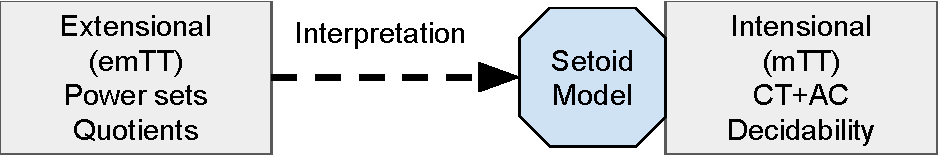
\includegraphics[trim= 0 0 0 0]{graph4}
               }

\end{frame}

\begin{frame}
\frametitle{Outline of Our Work}
\begin{block}{Work in Progress}
	\begin{itemize}
	\item	Type checkers for the two levels of the Minimalist Foundation 
			(implemented in $\lambda$Prolog).
	\item 	Implementation (in $\lambda$Prolog) of the interpretation from 
			the extensional level to the intensional level.
	\end{itemize}
\end{block}
\begin{block}{Future Works}
	\begin{itemize}
                \item   Formal validation of the interpretation (in Abella).
		\item	Proof assistant over the extensional level\\
                 (in $ELPI$ = $\lambda$Prolog + Constraint Programming)
		\item 	Code extraction at the intensional level.
	\end{itemize}
\end{block}

	\note[item]{ }



\end{frame}



\begin{frame}[fragile]
\frametitle{What Programming Language to Formalize a Theory?}
\begin{block}{Characteristics of $\lambda$-Prolog}
	\begin{enumerate}
		\item very high level language, usable by a logician/mathematician
		\item easy definition of structures with binders
		\item $\alpha$-equality and capture-avoiding substitution for free
		\item simple encoding of inference rules
		\item automatic management of non-determinism/backtracking
		\item simple reasoning on the programs (simple semantics)
	\end{enumerate}
\end{block}
\begin{block}{}
\emph{$\lambda$Prolog is the smallest extension to Prolog able to treat syntaxes with binders}
\end{block} 
\note{In particular we emphatise the ability to naturally work with binders }
\end{frame}

\begin{frame}[fragile]
\frametitle{Higher Order Logic Programming (HOLP)}
\begin{block}{$\lambda$Prolog = Prolog $\cup$ $\{\Rightarrow,\forall\}$ in queries}
\begin{columns}
 \column{0.5\textwidth}
		\begin{prooftree}
			\AxiomC{\begin{tabular}{c}[c]\\\vdots\\q\end{tabular}}
			\UnaryInfC{c =$>$ q}
		\end{prooftree}

   ~~~~~~~~~Locally scoped,\\ ~~~~~~\alert{hypothetical reasoning}

 \column{0.5\textwidth}
        \vspace{1.2cm}
	\begin{prooftree}
		\AxiomC{c$\{y/x\}$}\AxiomC{$y$ fresh}
		\BinaryInfC{pi x\bs c}
	\end{prooftree}

   ~~~~~~~~~~~~Generation of\\ ~~~~~~~~~~~~ \alert{fresh names}
\end{columns}
\end{block}

\begin{block}{}{HOAS + $\{\Rightarrow,\forall\}$ for entering binders in recursive definition}
 %$\texttt{b}$ is a binder of type $S \rightarrow T$ in HOAS\\
 %~~~~~~~\texttt{p~(b~F) :\!- pi x \bs q~x => q~(F x)}\\
 %$F~x$ is the body of the binder instantiated on $x$ fresh
\end{block}
\end{frame}

\begin{frame}[fragile]\frametitle{The Hello-World of $\lambda$Prolog}
%{
%\begin{block}{Example: $\lambda x. \lambda y. y x x$}
%	\begin{semiverbatim}
%		lam x \\ lam y \\ app (app y x) x
%	\end{semiverbatim}
%\end{block}}

%\begin{block}{Example: $\lambda x. \lambda y. y x x$}
%	\begin{semiverbatim}
%		lam \alert(x \\ lam \alert(y \\ app (app y x) x\alert)\alert)
%	\end{semiverbatim}
%\end{block}
\note[item]{Da rendere più chiaro con dei colori}
\note[item]{In $\lambda$Prolog is easy to formalize the simply typed $\lambda$-Calculus}
\note[item]{The binding and $\alpha$ equivalence are handled by the language}
%\end{frame}



%\begin{frame}[fragile]\frametitle{The Hello-World of $\lambda$Prolog}
{\small
\begin{block}{Type-Checking for Simply Typed $\lambda$-calculus}
$$\frac{\Gamma \vdash M : A \to  B \quad \Gamma \vdash N : A}{\Gamma \vdash M N : B} \quad \quad \frac{\Gamma, x : A \vdash F~x : B}{\Gamma \vdash \lambda x. F~x : A \to B} \quad \quad \frac{(x:A) \in \Gamma}{\Gamma \vdash x : A}$$
\end{block}}

\begin{block}{Representation of Simply Typed $\lambda$-calculus}
	{\small \begin{semiverbatim}
			\textbf{type} app \hspace{1em} term -> term -> term.
			\textbf{type} lam \hspace{1em} (term -> term) -> term.
	\end{semiverbatim}}
\end{block}

\begin{block}{Type-Checking/Inference in $\lambda$Prolog}
{\small
\begin{semiverbatim}
of (app M N) B :- of M (arr A B), of N A.
of (lam F) (arr A B) :- \alert{pi x\\ of x A =>} of (F x) B.
\end{semiverbatim}}
\end{block}
\note[item]{observations}
\note[item]{Inference rules map cleanly to $\lambda$Prolog clauses}
\note[item]{When a binder is met: generate fresh name, assume hypotheses, instantiate body, do recursion}
\note[item]{The third typing rule for free variables can use the assumptions introduced in the lambda rule by the => in the pi}
\end{frame}

\section{Type checkers for the two levels of the Minimalist Foundation}

\begin{frame}[fragile]\frametitle{Preliminary Work: Minor Changes to the Calculus}
\begin{block}{Syntax directed version of the rules }
 ~~~ From

  \begin{center}
	\begin{bprooftree}
		\AxiomC{$x \in A$}
		\AxiomC{$A = B$}
		\BinaryInfC{$x \in B$}
	\end{bprooftree}
	\begin{bprooftree}
		\AxiomC{$f \in \Pi_{x \in B}C(x)$}
		\AxiomC{$t \in B$}
		\BinaryInfC{$f~t \in C(t)$}
	\end{bprooftree}
   \end{center}

  ~~~ to

   \begin{center}
	\begin{bprooftree}
		\AxiomC{$f \in \Pi_{x \in B}C(x)$}
		\AxiomC{$t \alert{\in=} B$}
		\BinaryInfC{$f~t \in C(t)$}
	\end{bprooftree}
   \end{center}
\end{block}

\begin{block}{Deterministic equality check}
 From
  \begin{bprooftree}
   \AxiomC{$(\lambda_{x \in B} C(x))~t = C(t)$}
  \end{bprooftree}\\
 to~~~~~
  \begin{bprooftree}
   \AxiomC{$(\lambda_{x \in B} C(x))~t \rhd C(t)$}
  \end{bprooftree}
 and
  \begin{bprooftree}
   \AxiomC{$(s = t) := s \rhd^* \!\! \,^*\!\!\lhd t$}
  \end{bprooftree}
\end{block}
\end{frame}

\begin{frame}[fragile]\frametitle{Preliminary Work: Major Changes to the Calculus}
\begin{block}{Problem: proofs are not recorded at the extensional level}
 \begin{center}{\small
			\begin{bprooftree}
				\AxiomC{$true \in  Eq(C,c,d)$}
				\UnaryInfC{$c = d \in C$}
			\end{bprooftree}
			\begin{bprooftree}
                         \AxiomC{$true \in B$\hspace{-1em}}
                         \AxiomC{$true \in C$\hspace{-1em}}
                         \AxiomC{$B~ \textsl{props}$\hspace{-1em}}
                         \AxiomC{$C~ \textsl{props}$}
                         \QuaternaryInfC{$true \in B \wedge C$}
			\end{bprooftree}
 }\end{center}
\end{block}
\begin{block}{Discarded solution}
 The typechecker takes the whole \alert{derivation} in input.\\

 The datatype for the derivation is yet another typed $\lambda$-calculus.
\end{block}

\begin{block}{Partial solution}
 %For first order logic rules we keep the proof term like in the intensional level.\\
  Keep proof terms as in the intensional level.\\
 %The user can still just be shown a $true$ because of proof irrelevance.\\
 To a user we can still show $true$  because of proof irrelevance.\\
 It does not solve the problem of the $conv$ rule.
\end{block}
\end{frame}

\begin{frame}[fragile]\frametitle{Preliminary Work: Major Changes to the Calculus}
\begin{block}{Full solution: deterministic equality check in the ext. level}
 ~~~From arbitrary conversion proofs \note[item]{that would trigger general proof search}
\begin{center}
			\begin{bprooftree}
				\AxiomC{$true \in  Eq(C,c,d)$}
				\UnaryInfC{$c = d \in C$}
			\end{bprooftree}
\end{center}
 ~~~to contextual closure + context lookup rule
\begin{center}
			\begin{bprooftree}
				\AxiomC{$(x \in  Eq(C,c,d)) \in \Gamma$}
				\UnaryInfC{$c = d \in C$}
			\end{bprooftree}
\end{center}
 ~~~and new LetIn term constructor
\begin{center}
			\begin{bprooftree}
				\AxiomC{$p \in P$}
				\AxiomC{$t \in T\, [x \in P]$}
				\BinaryInfC{$let\; x := p \in P \; in \; t \in T$}
			\end{bprooftree}
\end{center}
\end{block}
\end{frame}


\begin{frame}[fragile]\frametitle{Preliminary Work: Changes for Code Reuse}
{\small
\vspace{-0.2em}
\begin{block}{$\Pi$ Introduction rule}	
	\begin{bprooftree}
		\AxiomC{$B\ set$}
		\AxiomC{$c(x) \in C(x)\ \alert{[x \in B]}$}
		\AxiomC{$C(x)\ set\  \alert{[x \in B]}$}
		\TrinaryInfC{$\lambda x^B .c(x) \in \Pi_{x\in B}C(x)$}
	\end{bprooftree}
	\begin{semiverbatim}
		of (lambda B F) (setPi B C) \cblue{IE} :-
		\ \ isType B _ \cblue{IE},
		\ \ (pi x\\ \alert{locDecl x B} => isType (C x) _ \cblue{IE})
		\ \ pi x\\ \alert{locDecl x B} => of (F x) (C x) \cblue{IE}.
	\end{semiverbatim}
\end{block}

\begin{block}{$\Pi$ Formation rule}	
	\begin{columns}
		\column{0.45\textwidth}
		\begin{bprooftree}
			\AxiomC{$B\  set$}
			\AxiomC{$C(x)\ set\  [x \in B]$}
			\BinaryInfC{$\Pi_{x\in B}C(x)\ set$}
		\end{bprooftree}
		\column{0.45\textwidth}
		\begin{bprooftree}
			\AxiomC{$B\  col$}
		\AxiomC{$C(x)\ col\  [x \in B]$}
		\BinaryInfC{$\Pi_{x\in B}C(x)\ col$}
		\end{bprooftree}
	\end{columns}
	\begin{semiverbatim}
		isType (setPi B C) \cblue{KIND3} IE :-
		\ \ isType B \cblue{KIND1} IE, 
		\ \ pi x\ locDecl x B  => isType (C x) \cblue{KIND2} IE,
		\ \ \cblue{pts\_pi KIND1 KIND2 KIND3}.
	\end{semiverbatim}
\end{block}
}
\note[item]{Here we can see that the first rule correctly propagates the intensionality or extensionality through  the parameter IE}
\note[item]{In the second rule we use an auxiliary predicate to unify the inferred Kinds of for B and C(x)}
\note[]{}
\note{TODO: in particolare nelle regole di mTT/emTT il Pi va solo da set a set (e quindi anche props)
	 esiste mTT${}^{dp}$ dove possono prendere collezioni ma non lo permette mai nel livello estensionale.
	 Sarebbe da fare la scelta tra modificare il codice/la regola o notare che usiamo regole più permissive. opterei per quest'ultima.
}
\end{frame}



\begin{frame}{}\frametitle{Typechecking and future works}

\begin{block}{Typechecking}
\begin{itemize}
	\item Code reuse between levels.\note[item]{via a boolean parameter}
	\item Code reduction via PTS-style.\note[item]{via pts unification}
		\note[item]{non sono sicuro che questo sia un modo appropriato di usare i pts}
	\item Extremely modular code.
		\note[item]{We can add predicates and type constructors incrementally}
	%\item Judgemental equality via computational conversion.
	%	\note[item]{which is decidable at the extensional level}
\end{itemize}
\end{block}
\begin{block}{Future works}
\begin{itemize}
        \item Complete and debug all the rules.
	\item The changes to the calculi have to be validated
	\item The $\xi$-rule at the intentional level must be removed.\\
          Requires a syntax directed version of explicit substitutions.
		\note[item]{In the scope of our work it should make no difference}
		\note[item]{\alert{TODO: la maietti afferma nel suo articolo che la xi-rule sia incompatibile con proof-as-programs (CT+AC). non mi è sufficientemente chiaro come proofs-as-programs e CodeExtraction siano distinti}}
\end{itemize}
\end{block}
\end{frame}

\section{Interpreting the extensional level in the intensional level}

\begin{frame}\frametitle{Design of the Interpretation}
\begin{block}{The Interpretation in a Nutshell}
\begin{itemize}
	\item In the Minimalist Foundation types are interpreted in dependent setoids.
	\item The interpretation on types is defined by structural recursion.
	\item For simple types (the singleton, the empty set, naturals) the setoid equality is the intensional propositional equality
        \item The equality of functions imposes the $\xi$ rule
        \item Proof irrelevance is imposed by the interpretation
	%\item The interpretation is defined on closed $\lambda$-terms. 
        \item Lack of impredicative quantifications avoids user-defined
         type equalities: this is NOT homotopy type theory
\end{itemize}
\end{block}
\end{frame}

\begin{frame}\frametitle{Design of the Interpretation}
\begin{block}{The Interpretation is Rich and Complex}
\begin{itemize}
        \item Requires lots of (proof) terms to be defined by meta-level
         recursion on types, terms and derivations of equalities
         \begin{itemize}
          \item proofs of reflexivity, symmetry, transitivity
          \item proofs that equivalences behave as congruences for every user defined function
          \item canonical isomorphisms between interpretation of extensionally
           equal types
          \item proofs that they are indeed isomorphisms
          \item \ldots
         \end{itemize}
     	 \item We are unable to directly use the proof of the paper as they are often given in categorical terms.
%        \item In the paper most proof terms are provided implicitly
%         \begin{itemize}
%           \item as computational content of intuitionistic proofs
%           \item via categorical completions
%         \end{itemize}
\end{itemize}
\end{block}
\end{frame}


\begin{frame}[fragile]{The Main Issue}
 \begin{block}{Subsumption becomes coercions}
 \begin{itemize}
	\item Equality used to fix mismatching (extensionally convertible) types must become term translation.
        
	\begin{bprooftree}
		\AxiomC{$x \in A$}
		\AxiomC{$A = B$}
		\BinaryInfC{$x \in B$}
	\end{bprooftree}
        becomes
	\begin{bprooftree}
		\AxiomC{$x \in A$}
		\AxiomC{$A \mathcal{R} B$}
		\BinaryInfC{$\sigma x  \in B$}
	\end{bprooftree}
        \item $\sigma$ is defined by recursion also over the proof of $A = B$ (compring the missing derivations of $Eq(T,c,d)$)\\
              Luckily we made proof search deterministic via let-ins and restricting to congruence rules and context lookup
	\item An example of an extensionally well typed term with mismatching types
		\(\forall_{x \in\mathds1} 
			\forall_{\alert{f \in {(x =_{\mathds1} \bigstar) \rightarrow {\mathds1}}}} 
				( \bigstar =_{\mathds1} x )  \Rightarrow \cblue{f(rfl(\bigstar))} =_{\mathds1} \cgreen{f(rfl(\bigstar))} \)
%\item To implement the functionality of the elimination rule for the extentional propositional equality \[\begin{bprooftree}
%\AxiomC{$true \in  Eq(C,c,d)$}
%\UnaryInfC{$c = d \in C$}
%\end{bprooftree}\] we use context lookup provided by the language together with a let-in construct.
\end{itemize}
		\note[item]{The support is just an intensional type and the equality is an intensional proposition}
			\note[item]{which are more natural to work with compared to full derivations}
 \end{block}
\end{frame}

\begin{frame}[fragile]{Interpretation of Types}{}{}{}{\small
	\begin{semiverbatim}
		forall singleton x0 \\ 
		\ \ forall \alert{(colSigma ({fun (propId singleton x0 star) singleton}) x1 \\
		\ \ forall (propId singleton x0 star) x2 \\ 
		\ \ forall (propId singleton x0 star) x3 \\ 
		\ \ forall (propId singleton star star) x4 \\ 
		\ \ propId singleton (fun_app x1 x2) (fun_app x1 x3))} x1 \\
		forall (propId singleton star x0) x2 \\ propId singleton
		\cblue{(fun_app (elim_colSigma x1 (x3 \\ 
		\ \ \ \ fun (propId singleton x0 star) singleton) x3 \\ x4 \\ x3)
		\ \ \ \ (impl_app (impl_app (forall_app (forall_app (impl_app 
		\ \ \ \ (forall_app (forall_app (k_propId singleton) star) x0) 
		\ \ \ \ x2) star) star) (id singleton star)) (id singleton star)))}
		\cgreen{(fun_app (elim_colSigma x1 (x3 \\ 
		\ \ \ \ fun (propId singleton x0 star) singleton) x3 \\ x4 \\ x3)
		\ \ \ \ (impl_app (impl_app (forall_app (forall_app (impl_app 
		\ \ \ \ (forall_app (forall_app (k_propId singleton) star) x0) 
		\ \ \ \ x2) star) star) (id singleton star)) (id singleton star)))}		
	\end{semiverbatim}
}
\end{frame}

\begin{frame}[fragile]{Auxiliary Predicates for the Interpretation}
\small\vspace{-0.2cm}
\begin{semiverbatim}
pippo (propEq T T1 T2) (propEq T T1' T2') (SIGMA) :- 
\ \ \ (pippoequ T1 T1' F1),
\ \ \ (pippoequ T2 T2' F2),
\ \ \ (trad T1 T1i),
\ \ \ (trad T2 T2i),
\ \ \ (trad T1' T1i'),
\ \ \ (trad T2' T2i'),
\ \ \ (trad T Ti),
\ \ \ SIGMA = x\\ impl_app ( 
\ \ \ \ \ impl_app ( forall_app ( forall_app ( impl_app ( forall_app ( 
\ \ \ \ \ forall_app (k_propId Ti) T1i) T1i') F1) T2i) T2i') F2)  x.
\end{semiverbatim}
\note[item]{pippo take 2 types that are extensionally convertible and produces a LambdaProlog function that transform an element of the first type in an element of the second type}
\note[item]{it is the equivalent of the $\sigma$s in Maietti's work}
\note[item]{pippoequ insted produces a an intensional proof of the setoid equality of its two arguments}
\begin{semiverbatim}
	pippoequ (fun_app F X1) (fun_app F X2) H :-
	\ \ pippoequ X1 X2 G,
	\ \ trad F F',
	\ \ P2F' = elim_colSigma F' _ (x\\ y\\ y),
	\ \ trad X1 X1',
	\ \ trad X2 X2',
	\ \ H = forall_app (forall_app (forall_app P2F' X1') X2') G. 
\end{semiverbatim}
\end{frame}

\section{Conclusions and Future Works}

\begin{frame}[fragile]{Conclusions}
%  Implementing the Minimalist Foundation is very time consuming
%   \begin{itemize}
%    \item Simple type-checking rules
%    \item Lot of them
%    \item Tons of terms to be provided in the translation
%   \end{itemize}
%
%  ~\\

  Implementing the Minimalist Foundation is non trivial
   \begin{itemize}
   	\item Many different type constructors and rules.
    \item Many terms need to be provided during the interpretation.
    \item Extensional type theories pose issues to the implementors.
    \item Implementation choices impact the calculus.
    \item The good properties must be preserved.
   \end{itemize}
	
	~\\
	
	But the constrained nature of the theory helps
	\begin{itemize}
		\item Structural recursion on types is facilitated by their very rigid structure.
		\item The propositional equality (int./ext.) is the only type constructor that directly takes terms as arguments.
		
	\end{itemize}
\end{frame}

\begin{frame}[fragile]{Conclusions and Future Works}\small
  $\lambda$Prolog was a great choice
  \begin{itemize}
   \item Takes away the pain due to binders, $\alpha$-conversion,
    capture avoiding substitution, etc.
   \item The code is in 1-1 relation with the new syntax oriented version of
    the formal inference rules.
   \item Joint Bologna/INRIA effort to combine $\lambda$Prolog with Constraint
     Programming to smoothly transition to proof assistant implementation.
  \end{itemize}
%\end{frame}
%
%\begin{frame}[fragile]{Future Works}
In the future we wish to extend our work
 \begin{itemize}
  \item Complete and validate (in Abella) the type checkers and interpretation.
%  \item Formally prove soundness of the interpretation in Abella.
  \item Implement code extraction for the intensional level.
  \item Implement a proof assistant for the extensional level.
  \item Validate the proof assistant formalizing Sambin's Basic Picture book
   (porting proofs from Matita).
 \end{itemize}
\end{frame}

\end{document}
